\section{Что мы будем понимать под исследованиями?}

\epigraph{Проблемы начинаются не тогда, когда имея в виду одно используют разные слова, а когда используя одни и теже слова имеют в виду разное.}{хорошо бы найти оригинал}

Проведение исследований неразрывно связано с понятиями -- данные, информация, знания. Эти термины всем знакомы, кажутся самодостаточными и очевидными. Их определения и различные трактовки можно легко найти в интернете, например на \url{https://ru.wikipedia.org/}.

\marginpar{
        \href{https://ru.wikipedia.org/wiki/информация}{Информация} 
        \newline
        
\includegraphics[scale=0.4]{pics/qr_wikipedia_information.png} 
        \newline
        \href{https://ru.wikipedia.org/wiki/данные}{Данные} 
        \newline
        
\includegraphics[scale=0.4]{pics/qr_wikipedia_data.png}
    }

Следствием распространённости этих понятий является многообразие их значений и интерпретаций в различных областях деятельности. Приведём здесь одну из интерпретаций, которой будем в дальнейшем придерживаться (\ref{ris:data_info_chart_1}. ). 

\begin{figure}[h!]
	\begin{center}
		

\tikzset{every picture/.style={line width=0.75pt}} %set default line width to 0.75pt        

\begin{tikzpicture}[x=0.75pt,y=0.75pt,yscale=-1,xscale=1]
%uncomment if require: \path (0,239); %set diagram left start at 0, and has height of 239

%Rounded Rect [id:dp8355723819738923] 
\draw [fill={rgb, 255:red, 184; green, 233; blue, 134 }  ,fill opacity=1 ]  (98,119.5) .. controls (98,115.08) and (101.58,111.5) .. (106,111.5) -- (202.97,111.5) .. controls (207.39,111.5) and (210.97,115.08) .. (210.97,119.5) -- (210.97,143.5) .. controls (210.97,147.92) and (207.39,151.5) .. (202.97,151.5) -- (106,151.5) .. controls (101.58,151.5) and (98,147.92) .. (98,143.5) -- cycle ;
%Rounded Rect [id:dp6680308810096447] 
\draw [fill={rgb, 255:red, 184; green, 233; blue, 134 }  ,fill opacity=1 ]  (270,119.5) .. controls (270,115.08) and (273.58,111.5) .. (278,111.5) -- (374.97,111.5) .. controls (379.39,111.5) and (382.97,115.08) .. (382.97,119.5) -- (382.97,143.5) .. controls (382.97,147.92) and (379.39,151.5) .. (374.97,151.5) -- (278,151.5) .. controls (273.58,151.5) and (270,147.92) .. (270,143.5) -- cycle ;
%Straight Lines [id:da6784338312341602] 
\draw    (211,131) -- (268,131) ;
\draw [shift={(268,131)}, rotate = 180] [color={rgb, 255:red, 0; green, 0; blue, 0 }  ][line width=0.75]    (10.93,-3.29) .. controls (6.95,-1.4) and (3.31,-0.3) .. (0,0) .. controls (3.31,0.3) and (6.95,1.4) .. (10.93,3.29)   ;

% Text Node
\draw (127,125) node [anchor=north west][inner sep=0.75pt]   [align=left] {Данные};
% Text Node
\draw (286,125) node [anchor=north west][inner sep=0.75pt]   [align=left] {Информация};

% Text Node
\draw (90,160) node [anchor=north west][inner sep=0.75pt]   [align=left] {То, что зафиксировано};
% Text Node
\draw (272,160) node [anchor=north west][inner sep=0.75pt]   [align=left] {То, что обработано};


\end{tikzpicture}

		\caption{Связь данных и информации}
		\label{ris:data_info_chart_1}
	\end{center}
\end{figure}

Под данными мы будем понимать совокупность сведений, зафиксированных на определенном носителе в форме пригодной для постоянного хранения обработки и интерпретации. Например замеры давления на приеме УЭЦН записанные в базу данных - это данные. Главное, что они записаны и к ним можно получить доступ при необходимости. 
Под информацией мы будем понимать результат преобразования и анализа данных направленный на практическую деятельность -- на принятие решений. Хотя информация должна обрести некоторую форму представления, то есть превратиться в данные, чтобы ей можно было обмениваться, информация есть в первую очередь интерпретация (смысл) такого представления. Информация всегда привязана к практической деятельности. Без применения, хотя бы потенциального, информация превращается в данные. 

Инженерная деятельность подразумевает постоянные действия для решения поставленных задач. Для нефтяного инжиниринга это эксплуатация месторождений углеводородов -- бурение скважине, проведение геолого-технических мероприятий. Действия или решения требуют необратимой траты ресурсов -- времени, материалов, денег. Из за ограниченности ресурсов возникает необходимость тщательного планирования действий -- принятия решений о необходимости действий. Мы часто будем использовать термин принятие решений и говорить о лице принимающем решение (ЛПР) для обозначения практической деятельности. Принятие решений -- это тот рубеж, который является целью исследований. Для принятия решений строятся модели, собираются данные и генерируется информация. 


Цепочку связи данных, информации и принятия решений можно отобразить схеме (рисунок  \ref{ris:data_info_decision_chart_1}). 

\begin{figure}[h!]
	\begin{center}
		

\tikzset{every picture/.style={line width=0.75pt}} %set default line width to 0.75pt        

\begin{tikzpicture}[x=0.75pt,y=0.75pt,yscale=-1,xscale=1]
%uncomment if require: \path (0,300); %set diagram left start at 0, and has height of 300

%Rounded Rect [id:dp2235462280724534] 
\draw  [fill={rgb, 255:red, 184; green, 233; blue, 134 }  ,fill opacity=1 ] (135.2,68) .. controls (135.2,63.58) and (138.78,60) .. (143.2,60) -- (227.97,60) .. controls (232.39,60) and (235.97,63.58) .. (235.97,68) -- (235.97,92) .. controls (235.97,96.42) and (232.39,100) .. (227.97,100) -- (143.2,100) .. controls (138.78,100) and (135.2,96.42) .. (135.2,92) -- cycle ;
%Rounded Rect [id:dp17536142021697776] 
\draw  [fill={rgb, 255:red, 184; green, 233; blue, 134 }  ,fill opacity=1 ] (293,68) .. controls (293,63.58) and (296.58,60) .. (301,60) -- (388.97,60) .. controls (393.39,60) and (396.97,63.58) .. (396.97,68) -- (396.97,92) .. controls (396.97,96.42) and (393.39,100) .. (388.97,100) -- (301,100) .. controls (296.58,100) and (293,96.42) .. (293,92) -- cycle ;
%Straight Lines [id:da11139667469680425] 
\draw    (264.92,45.28) -- (264.92,78) ;
\draw [shift={(264.92,80)}, rotate = 270] [color={rgb, 255:red, 0; green, 0; blue, 0 }  ][line width=0.75]    (10.93,-3.29) .. controls (6.95,-1.4) and (3.31,-0.3) .. (0,0) .. controls (3.31,0.3) and (6.95,1.4) .. (10.93,3.29)   ;
%Rounded Rect [id:dp3985813066419075] 
\draw  [fill={rgb, 255:red, 184; green, 233; blue, 134 }  ,fill opacity=1 ] (457,68) .. controls (457,63.58) and (460.58,60) .. (465,60) -- (594.52,60) .. controls (598.94,60) and (602.52,63.58) .. (602.52,68) -- (602.52,92) .. controls (602.52,96.42) and (598.94,100) .. (594.52,100) -- (465,100) .. controls (460.58,100) and (457,96.42) .. (457,92) -- cycle ;
%Straight Lines [id:da985211792743889] 
\draw    (397.4,80) -- (455.11,80) ;
\draw [shift={(457.11,80)}, rotate = 180] [color={rgb, 255:red, 0; green, 0; blue, 0 }  ][line width=0.75]    (10.93,-3.29) .. controls (6.95,-1.4) and (3.31,-0.3) .. (0,0) .. controls (3.31,0.3) and (6.95,1.4) .. (10.93,3.29)   ;
%Rounded Rect [id:dp8115508928060304] 
\draw  [fill={rgb, 255:red, 245; green, 166; blue, 35 }  ,fill opacity=1 ] (210.11,13.28) .. controls (210.11,8.86) and (213.69,5.28) .. (218.11,5.28) -- (311.73,5.28) .. controls (316.15,5.28) and (319.73,8.86) .. (319.73,13.28) -- (319.73,37.28) .. controls (319.73,41.7) and (316.15,45.28) .. (311.73,45.28) -- (218.11,45.28) .. controls (213.69,45.28) and (210.11,41.7) .. (210.11,37.28) -- cycle ;
%Straight Lines [id:da5256470314414583] 
\draw    (235.97,80) -- (290.71,80) ;
\draw [shift={(292.71,80)}, rotate = 180] [color={rgb, 255:red, 0; green, 0; blue, 0 }  ][line width=0.75]    (10.93,-3.29) .. controls (6.95,-1.4) and (3.31,-0.3) .. (0,0) .. controls (3.31,0.3) and (6.95,1.4) .. (10.93,3.29)   ;

% Text Node
\draw (186.09,79.95) node   [align=left] {Данные};
% Text Node
\draw (343.91,79.95) node   [align=left] {Информация};
% Text Node
\draw (529.76,80) node   [align=left] {Принятие решений};
% Text Node
\draw (264.81,24.62) node   [align=left] {Исследование};


\end{tikzpicture}
		\caption{Связь данных, информации и принятия решений}
		\label{ris:data_info_decision_chart_1}
	\end{center}
\end{figure}

Схема показывает, что информация напрямую связана с принятием решений. Если мы не понимаем зачем необходима информация -- на принятие какого решения она работает, то она может оказаться бессмысленной. В приведенной схеме процесс преобразования данных в информацию можно назвать исследованием. 
Цель исследования -- обеспечить процесс принятия решений информаций. И аналогично информации -- исследование имеет смысл только если направлено на принятие решений. 
\marginpar{
	\href{https://ru.wikipedia.org/wiki/исследование}{Исследование} 
	
\includegraphics[scale=0.4]{pics/qr_wikipedia_investigation.png} } 
Схему можно еще дополнить добавив в нее инструмент для преобразования данных в информацию и принятия решений на основе информации -- модель. Чаще всего имеются в виду математические модели в виде компьютерных алгоритмов. Именно их мы будет использовать, но на их месте могут быть и другие модели (например интуиция лица принимающего решения или его опыт). 

\begin{figure}[h!]
	\begin{center}
		

\tikzset{every picture/.style={line width=0.75pt}} %set default line width to 0.75pt        

\begin{tikzpicture}[x=0.75pt,y=0.75pt,yscale=-1,xscale=1]
%uncomment if require: \path (0,300); %set diagram left start at 0, and has height of 300

%Rounded Rect [id:dp597190226460943] 
\draw   (113.2,151) .. controls (113.2,146.58) and (116.78,143) .. (121.2,143) -- (208.97,143) .. controls (213.39,143) and (216.97,146.58) .. (216.97,151) -- (216.97,175) .. controls (216.97,179.42) and (213.39,183) .. (208.97,183) -- (121.2,183) .. controls (116.78,183) and (113.2,179.42) .. (113.2,175) -- cycle ;
%Rounded Rect [id:dp3409304527040422] 
\draw   (274,151) .. controls (274,146.58) and (277.58,143) .. (282,143) -- (378.97,143) .. controls (383.39,143) and (386.97,146.58) .. (386.97,151) -- (386.97,175) .. controls (386.97,179.42) and (383.39,183) .. (378.97,183) -- (282,183) .. controls (277.58,183) and (274,179.42) .. (274,175) -- cycle ;
%Straight Lines [id:da9955922595564108] 
\draw    (216,163) -- (273.2,163) ;
\draw [shift={(275.2,163)}, rotate = 180] [color={rgb, 255:red, 0; green, 0; blue, 0 }  ][line width=0.75]    (10.93,-3.29) .. controls (6.95,-1.4) and (3.31,-0.3) .. (0,0) .. controls (3.31,0.3) and (6.95,1.4) .. (10.93,3.29)   ;
%Rounded Rect [id:dp45297167935805027] 
\draw   (451,151) .. controls (451,146.58) and (454.58,143) .. (459,143) -- (574.2,143) .. controls (578.62,143) and (582.2,146.58) .. (582.2,151) -- (582.2,175) .. controls (582.2,179.42) and (578.62,183) .. (574.2,183) -- (459,183) .. controls (454.58,183) and (451,179.42) .. (451,175) -- cycle ;
%Straight Lines [id:da11147374736012572] 
\draw    (388.2,161.94) -- (447.2,162) ;
\draw [shift={(449.2,162)}, rotate = 180.06] [color={rgb, 255:red, 0; green, 0; blue, 0 }  ][line width=0.75]    (10.93,-3.29) .. controls (6.95,-1.4) and (3.31,-0.3) .. (0,0) .. controls (3.31,0.3) and (6.95,1.4) .. (10.93,3.29)   ;
%Rounded Rect [id:dp851243700176072] 
\draw   (211.2,209) .. controls (211.2,204.58) and (214.78,201) .. (219.2,201) -- (442.2,201) .. controls (446.62,201) and (450.2,204.58) .. (450.2,209) -- (450.2,233) .. controls (450.2,237.42) and (446.62,241) .. (442.2,241) -- (219.2,241) .. controls (214.78,241) and (211.2,237.42) .. (211.2,233) -- cycle ;
%Straight Lines [id:da1477687213170571] 
\draw    (245,200.5) -- (245.57,165) ;
\draw [shift={(245.6,163)}, rotate = 450.92] [color={rgb, 255:red, 0; green, 0; blue, 0 }  ][line width=0.75]    (10.93,-3.29) .. controls (6.95,-1.4) and (3.31,-0.3) .. (0,0) .. controls (3.31,0.3) and (6.95,1.4) .. (10.93,3.29)   ;
%Straight Lines [id:da9162736044666429] 
\draw    (419,199.5) -- (419.57,164) ;
\draw [shift={(419.6,162)}, rotate = 450.92] [color={rgb, 255:red, 0; green, 0; blue, 0 }  ][line width=0.75]    (10.93,-3.29) .. controls (6.95,-1.4) and (3.31,-0.3) .. (0,0) .. controls (3.31,0.3) and (6.95,1.4) .. (10.93,3.29)   ;

% Text Node
\draw (137,153.5) node [anchor=north west][inner sep=0.75pt]   [align=left] {Данные};
% Text Node
\draw (285,154.5) node [anchor=north west][inner sep=0.75pt]   [align=left] {Информация};
% Text Node
\draw (460,153.5) node [anchor=north west][inner sep=0.75pt]   [align=left] {Принятие решений};
% Text Node
\draw (304,212.5) node [anchor=north west][inner sep=0.75pt]   [align=left] {Модель};


\end{tikzpicture}

		\caption{Связь данных, информации, принятия решений и моделирования}
		\label{ris:data_model_chart_1}
	\end{center}
\end{figure}

Именно такого подхода мы будем придерживаться в курсе и данном пособии. Такое определение, хотя и несколько отличается от классических, обладает рядом преимуществ. Например позволяет оценить когда надо проводить исследования и сколько ресурсов на них можно потратить или увидеть как можно некоторые виды деятельности, изначально не направленные на получение информации, рассматривать в качестве исследований и извлечь из них дополнительную ценность.
 \marginpar{
 	\href{https://www.gazprom-neft.ru/press-center/sibneft-online/archive/2018-may/1589542/} {Газпром нефть. Цифровизация — это фундаментальный тренд}.
 	
\includegraphics[scale=0.4]{pics/qr_digitalization.png} }  
Например с развитием информационных технологий в нефтедобычи все больше информации о нормальной эксплуатации скважины накапливается в базах данных добывающих компаний. Эти данные содержат информацию о том как работают скважины и месторождения. Если их рассмотреть как исследования -- их можно преобразовать в информацию и использовать ее для принятия решений, например о проведении ГТМ, без необходимости траты ресурсов на проведение классических исследований. Это направление сейчас активно развивается в нефтяной промышленности под знамёнами цифровизации и в рамках курса будет неоднократно обсуждаться.

Подумайте как можно на приведённые схемы добавить категорию - знание? Как могут быть связаны исследования и знания?

\section{Ожидаемая ценность в условиях неопределённости -- EMV}

Исследования почти всегда идут рядом с неопределённостями различного вида. Неопределённости могут быть связаны с параметрами изучаемых объектов. Например планируя пробурить скважину, мы хотели бы знать ее дебит. Мы знаем, что дебит будет зависеть от проницаемости пласта, но проницаемость мы не знаем -- мы находимся в ситуации неопределённости. 

Мы  можем описать неопределённость проницаемости задав вероятные исходы для значения проницаемости. Пусть мы ожидаем, что величина проницаемости задаётся следующим распределением:

\begin{itemize}
	\item $k_1 = 10$ мД с вероятностью $P_1 = 0.2$; 
	\item $k_2 = 20$ мД с вероятностью $P_2 = 0.6$; 
	\item $k_3 = 30$ мД с вероятностью $P_3 = 0.2$. 
\end{itemize}

Если мы рассмотрим задачу строительства новой скважины на месторождении с заданными параметрами, тогда дебиты скважины могут оценены из выражения

\begin{equation}
	Q = \frac{kh}{18.41 \mu B} \frac{\Delta P}{  \left( ln\dfrac{r_e}{r_w} + S\right) }
	\label{eq:eq_q}
\end{equation}

$Q$ -- дебит скважины ожидаемый;

$k$ -- проницаемость пласта, мД;

$h$ -- мощность пласта, м;

$\mu$ -- вязкость нефти, сП;

$B$ -- объемный коэффициент нефти, м$^3$/м$^3$

$\Delta P$ -- депрессия на пласт, атм;

$r_e$ -- радиус контура дренирования скважины, м;

$r_w$ -- радиус скважины, м;

$S$ -- скин-фактор скважины, м;


а доход от эксплуатации скважины в течении периода времени  $\Delta T$

\begin{equation}
	MV = Q \cdot  \Delta T \cdot  Price_{oil} - Price_{well}
	\label{eq:eq_MV}
\end{equation}

где 

$MV$ -- доход от эксплуатации (monetary value);

$Q$ -- дебит скважины ожидаемый;
 
$\Delta T$ -- период времени за который проходит оценка;

$Price_{oil}$ -- стоимость единицы добычи нефти.

$Price_{well}$ -- стоимость строительства скважины

Тогда подставляя \eqref{eq:eq_q} в \eqref{eq:eq_MV} получим 

\begin{equation}
	MV = \alpha k - \beta
	\label{eq:eq_MV_2}
\end{equation}

где 

$$\alpha =  \Delta T \cdot  Price \cdot \frac{h}{18.41 \mu B} \frac{\Delta P}{  \left( ln\dfrac{r_e}{r_w} + S\right)}
$$ 

$$
\beta = Price_{well}
$$

параметры, который мы предполагаем постоянными в рамках данной модели. 

Тогда ожидаемую доходность с учётом неопределённости можно получить как математическое ожидание доходности с учётом заданного распределения. 

\begin{equation}
	EMV = \sum_{i} MV \cdot P_i 
\end{equation}

Величину ожидаемой доходности можно представить в виде графической диаграммы, приведённой на рисунке \ref{ris:chance_node}.

Чтобы более наглядно представить последующие рассуждения, приведём численный пример.Предположим, что величина $\alpha = 1$, $\beta = 15$. Размерности величин не указываем, но понимаем, что это некоторый финансовый показатель.  

Тогда получим для случая строительства скважины с приведёнными выше априорными показателями 

\begin{multline}
	EMV = \sum_{i} (\alpha k_i - \beta ) P_i = \\
	= (1 \cdot 10 - 15) \cdot 0.2 + (1 \cdot 20 - 15)\cdot 0.6 + (1 \cdot 30 - 15)\cdot 0.2 = 5
\end{multline}

Для заданный условий получаем $EMV =5 > 0$, что можно интерпретировать, что в среднем бурение скважины в этих условиях будет рентабельно.


\begin{figure}[h!]
	\tikzset{every picture/.style={line width=0.75pt}} %set default line width to 0.75pt        
	\centering
	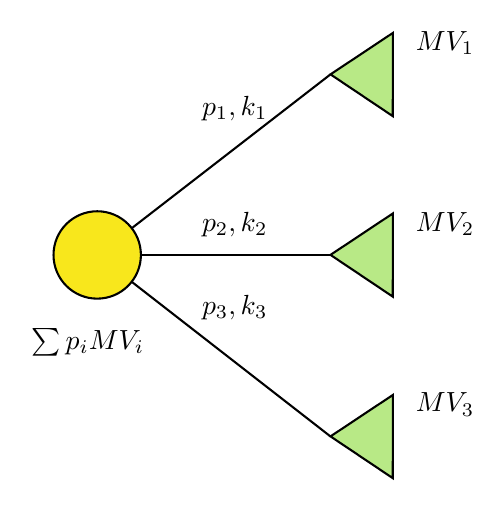
\begin{tikzpicture}[x=0.75pt,y=0.75pt,yscale=-1,xscale=1]
		%uncomment if require: \path (0,300); %set diagram left start at 0, and has height of 300
		
		%Straight Lines [id:da9914598188026227] 
		\draw    (125,128) -- (237.4,41) ;
		%Straight Lines [id:da8494600211227674] 
		\draw    (125,128) -- (237.4,215.45) ;
		%Straight Lines [id:da3455826146339449] 
		\draw    (125,128) -- (237.4,128) ;
		%Shape: Circle [id:dp4694470217534936] 
		\draw  [fill={rgb, 255:red, 248; green, 231; blue, 28 }  ,fill opacity=1 ] (103.95,128) .. controls (103.95,116.37) and (113.37,106.95) .. (125,106.95) .. controls (136.63,106.95) and (146.05,116.37) .. (146.05,128) .. controls (146.05,139.63) and (136.63,149.05) .. (125,149.05) .. controls (113.37,149.05) and (103.95,139.63) .. (103.95,128) -- cycle ;
		%Shape: Triangle [id:dp6993619331790251] 
		\draw  [fill={rgb, 255:red, 184; green, 233; blue, 134 }  ,fill opacity=1 ] (237.4,41) -- (267.48,21.01) -- (267.39,61.11) -- cycle ;
		%Shape: Triangle [id:dp5948591148628843] 
		\draw  [fill={rgb, 255:red, 184; green, 233; blue, 134 }  ,fill opacity=1 ] (237.4,127.97) -- (267.48,107.98) -- (267.39,148.08) -- cycle ;
		%Shape: Triangle [id:dp600205010959115] 
		\draw  [fill={rgb, 255:red, 184; green, 233; blue, 134 }  ,fill opacity=1 ] (237.4,215.42) -- (267.48,195.43) -- (267.39,235.53) -- cycle ;
		
		% Text Node
		\draw (174,50) node [anchor=north west][inner sep=0.75pt]    {$p_{1}, k_1$};
		% Text Node
		\draw (174,106) node [anchor=north west][inner sep=0.75pt]    {$p_{2}, k_2$};
		% Text Node
		\draw (174,146) node [anchor=north west][inner sep=0.75pt]    {$p_{3}, k_3$};
		% Text Node
		\draw (277,19) node [anchor=north west][inner sep=0.75pt]    {$MV_{1}$};
		% Text Node
		\draw (277,106) node [anchor=north west][inner sep=0.75pt]    {$MV_{2}$};
		% Text Node
		\draw (277,193) node [anchor=north west][inner sep=0.75pt]    {$MV_{3}$};
		% Text Node
		\draw (92,162) node [anchor=north west][inner sep=0.75pt]    {$\sum p_{i} MV_{i}$};
	\end{tikzpicture}
	\label{ris:chance_node}
	\caption{Графическое представление для вычисления ожидаемой доходности EMV}
\end{figure}

Здесь мы, следуя соглашения для отрисовки деревьев решений, в виде круга обозначили вероятностный узел -  выходами из которого являются ветви дерева, представляющие возможные дискретные исходы задаваемым природой или постановкой задачи - исходы на которые мы не можем повлиять. Конечные исходы обозначаем треугольниками. Каждая ветвь выходящая из вероятностного узла характеризуется вероятностью и значением проницаемости (для нашей задачи), каждый исход описывается величиной доходности при заданной вероятности. 

%надо доделать тут

\section{Ценность информации полученной в ходе исследований -- VOI}

Хорошим вопросом касательно любых исследований и даже шире -- любых расчётов и инженерных моделей -- является вопрос -- зачем всем этим надо заниматься? Задав этот вопрос, можно услышать много ответов. Часто говорят -- чтобы лучше изучить месторождение, чтобы определить параметры месторождения или скважины, чтобы рассчитать оптимальный режим работы скважины. Такие ответы верны, но в тоже время слишком расплывчаты. Попробуйте поставить себя на место главного инженера добывающего предприятия и оценить -- выделили бы вы ценные ресурсы молодому специалисту который предлагает лучше изучить какую-то скважину? 

Лица принимающие решения (главный инженер добывающего предприятия -- хорошая модель ЛПР для нашего курса) любят более конкретные обоснования как правило. Лучше всего экономические.

Один из ответов на вопрос -- "Зачем проводить исследования?" можно получить с использованием понятия ценности информации (Value of Information). 

\marginpar{
        \href{https://ru.wikipedia.org/wiki/ценность_информации}{Ценность информации} 
        
\includegraphics[scale=0.4]{pics/qr_wikipedia_VOI.png} 
        }

Согласно упрощённой версии этого подхода можно допустить, что ценность информации полученного в ходе исследования равна разнице в эффективности принятого решения с учётом этой информации и без ее учёта. 

\begin{equation}
	\label{eq:VOI}
	VOI = EMV_{inf}-EMV_{0} 
\end{equation}

Здесь $VOI$ - ценность информации, $EMV_{inf}$ - ожидаемая ценность принятого решения с учетом информации (estimated monetary value), $EMV_{0}$ - ожидаемая ценность принятого решения без учёта информации.

То есть ценность исследования, а следовательно и целесообразность его проведения (затрат ресурсов на его проведение) целиком зависит от эффективности принятых решений. 

Предположим, что для приведённых выше условий по априорному распределению проницаемости в пласте имеется возможность провести ГДИС и уточнить величины проницаемости. 

Например мы ожидаем, что после исследования мы сможем снизить неопределённость в проницаемости и тем самым уточнить дебит скважины после запуска.  

Предположим, что можно выделить два исхода распределения вероятности после проведения теста

Первый с вероятностью $p_1 = 0.5$

\begin{itemize}
	\item $k_1 = 10$ мД с вероятность $P_1 = 0.2$; 
	\item $k_2 = 15$ мД с вероятность $P_2 = 0.6$; 
	\item $k_3 = 20$ мД с вероятность $P_3 = 0.2$. 
\end{itemize}

Второй с вероятностью $p_1 = 0.5$

\begin{itemize}
	\item $k_1 = 20$ мД с вероятность $P_1 = 0.2$; 
	\item $k_2 = 25$ мД с вероятность $P_2 = 0.6$; 
	\item $k_3 = 30$ мД с вероятность $P_3 = 0.2$. 
\end{itemize}

\begin{figure}[h!]
	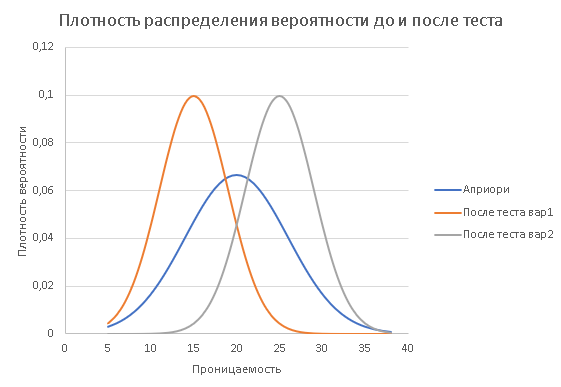
\includegraphics[width= 15cm]{pics_2/norm_distribution_ex1.png} 
	\label{fig:sample2}
	\caption{Иллюстрация к уточнению проницаемости в ходе исследований}
\end{figure}

Такой подход является явным упрощением. По приведённым ссылкам можно найти и другие подходы, где в частности предлагается учесть и менее явные последствия. Но его преимущество как раз в простоте. Он позволяет количественно оценить эффект от проведения исследований, соотнести его с затратами на проведение исследований и построить критерий принятия решений, который уже можно далее обсуждать и улучшать. 


Существует много подходов к построению критерия принятия решений о необходимости проведения исследований [ссылка на making good decisions]. Мы рассмотрим один из них, широко применяемый в различных областях деятельности, особенной в экономике и компьютерных науках - метод построения деревьев решений. \cite{AL_appl_patt_2007}

\section{Деревья решений для планирования исследований}

% translation from https://github.com/SilverDecisions/SilverDecisions/wiki/1.-Decision-tree-model
Последовательность и неопределенность присущи практическому принятию решений. Первое означает, что лица, принимающие решения, должны рассматривать многоступенчатые стратегии, охватывающие несколько действий, следующих друг за другом, а не только одно действие. Вторая означает, что отдача, получаемая лицами, принимающими решения, зависит не только от действий, но и от внешних событий ( состояний мира), которые часто могут быть восприняты как случайные. Действия и реакции обычно переплетаются, что еще больше усложняет картину. Деревья решений используются в качестве модели, помогающей обнаружить, понять и передать структуру таких проблем, связанных с принятием решений.

Ниже представлено простое дерево решений, созданное с помощью программы SilverDecisions (файл SilverDecisions, содержащий это дерево, можно запустить \href{http://silverdecisions.pl/SilverDecisions.html?LOAD_SD_TREE_JSON=https://raw.githubusercontent.com/gubkin-rienm/isp/master/data/decision_tree/simple_invest_decision.json}{здесь}).
\marginpar{
        ссылку там есть - надо сделать QR на нее
        }
%\urldef{\myurl}{http://silverdecisions.pl/SilverDecisions.html?LOAD_SD_TREE_JSON=https://raw.githubusercontent.com/gubkin-rienm/isp/master/data/decision_tree/simple_invest_decision.json}

\begin{figure}[h!]
	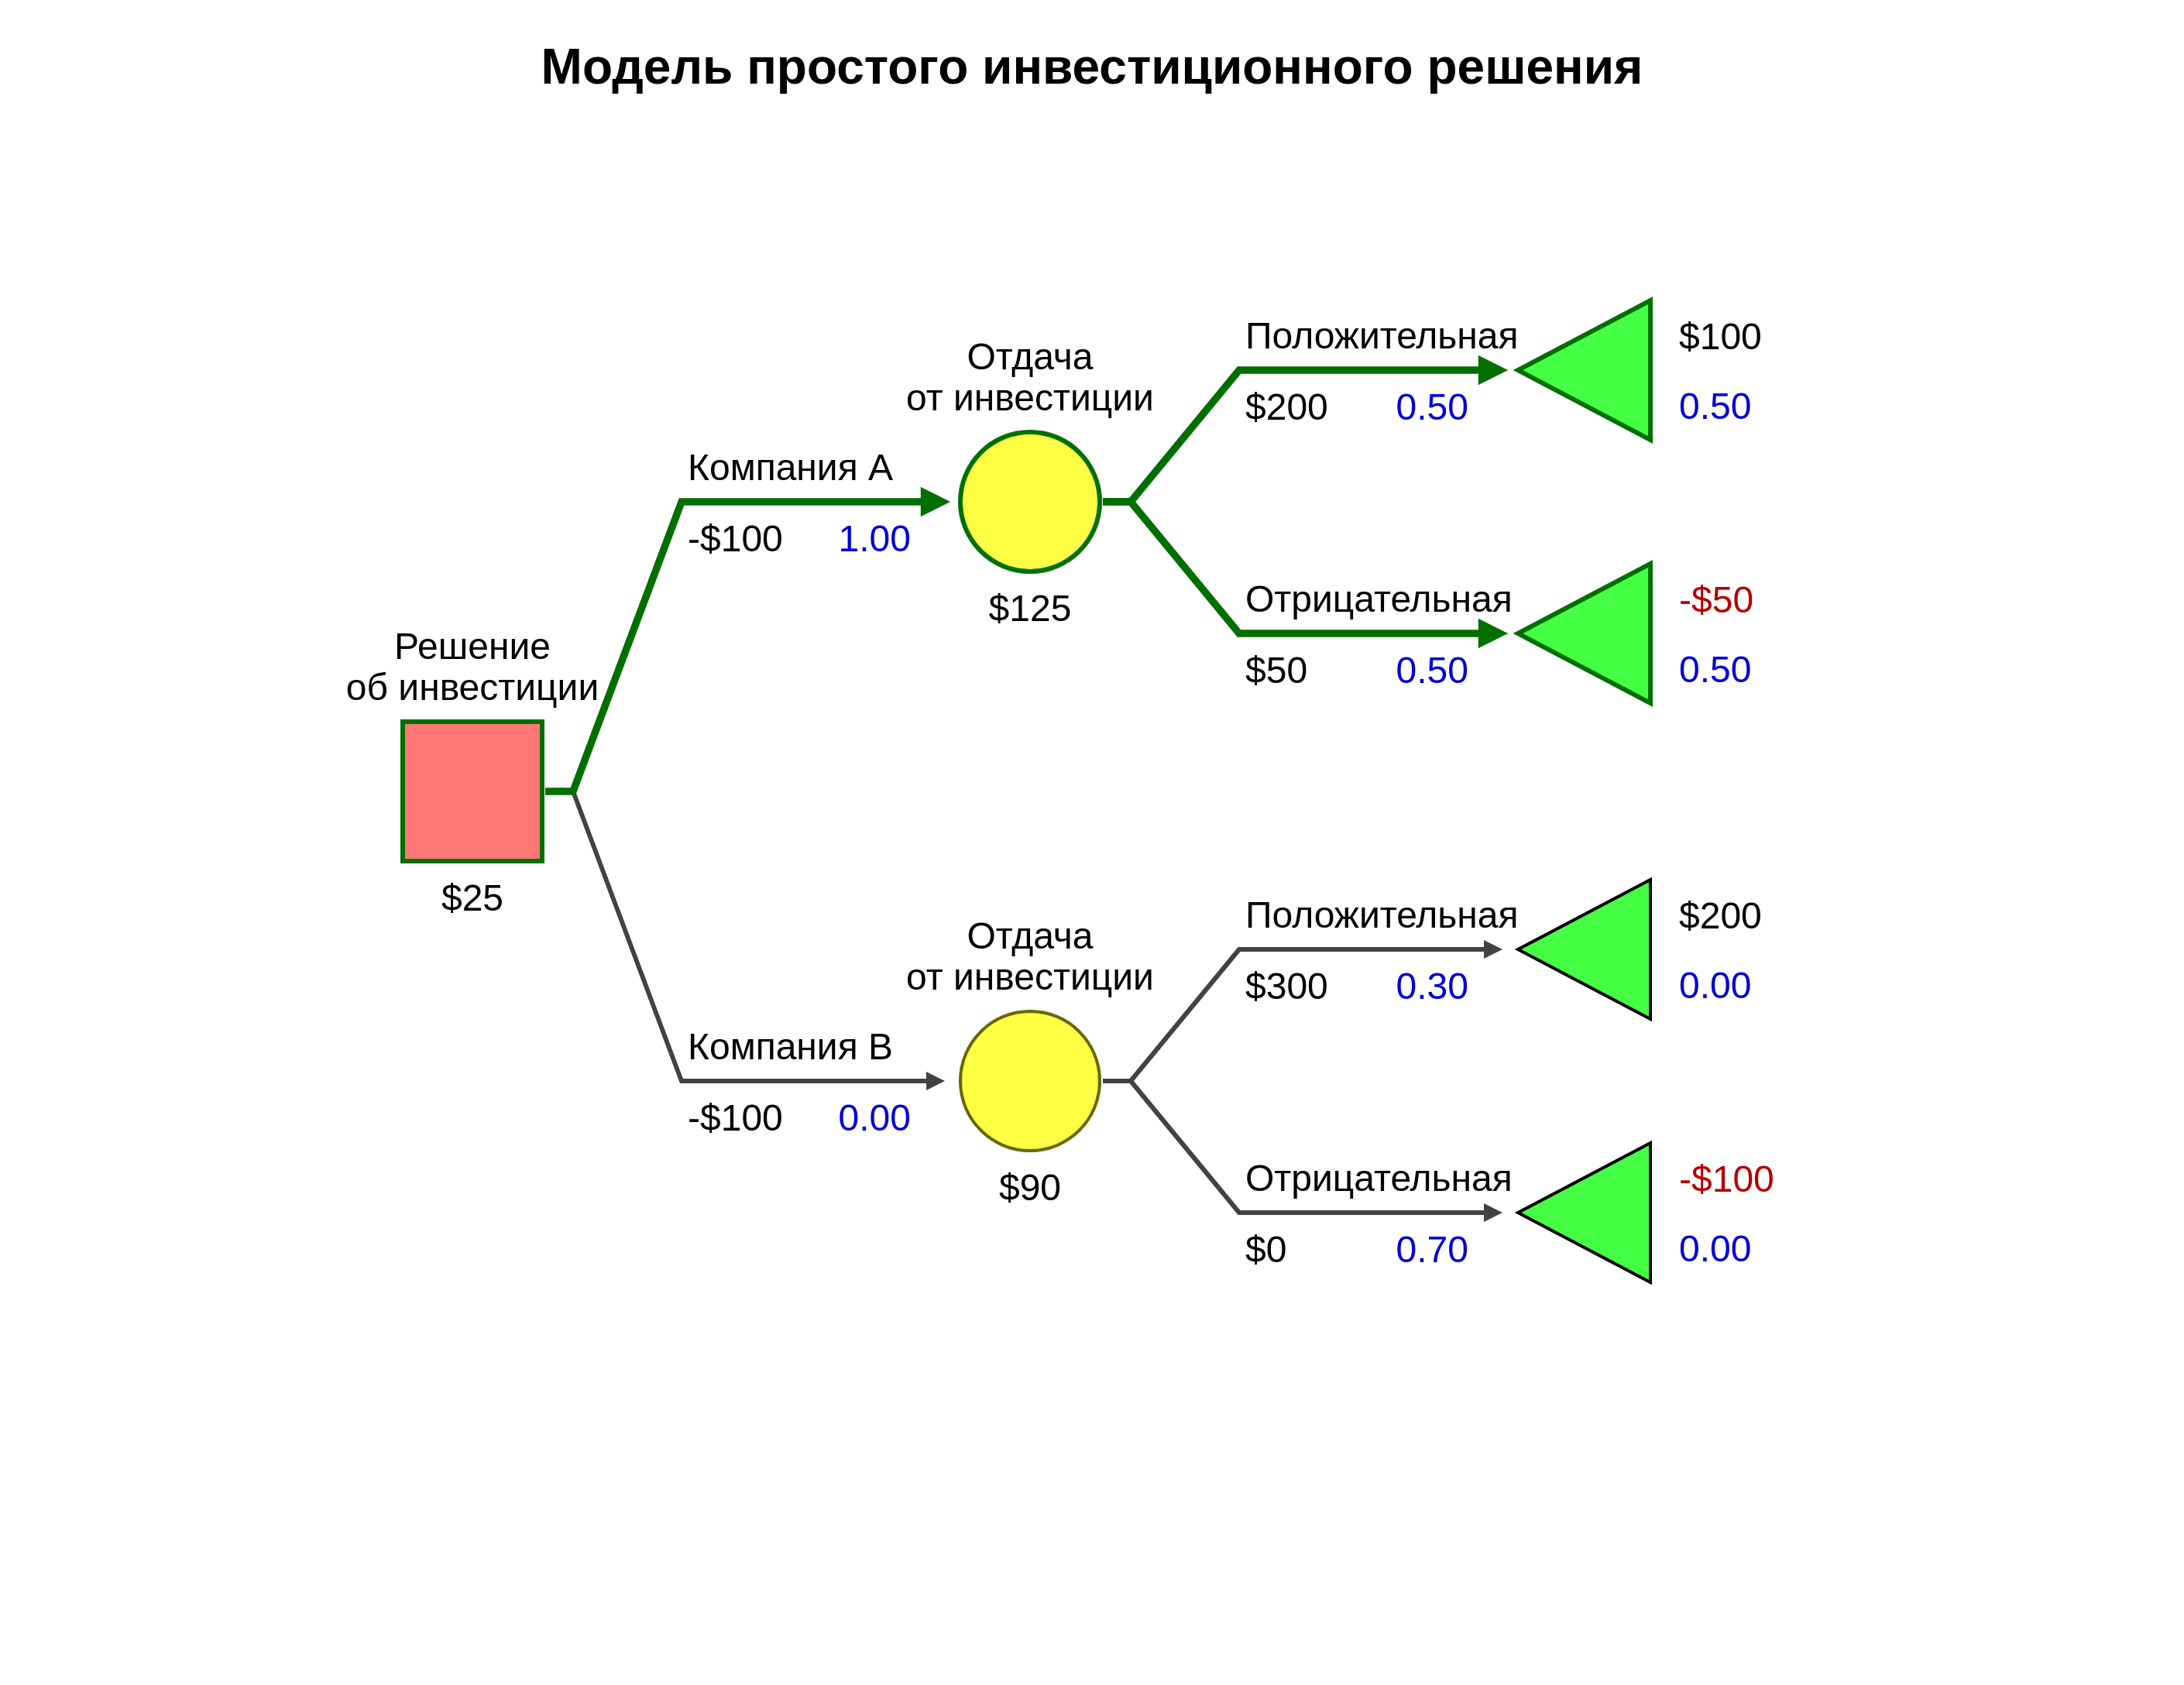
\includegraphics[width= 15cm]{pics/simple_decision_tree_1.png} 
	\label{fig:sample}
	\caption{Простое дерево решений}
\end{figure}

Модель дерева решений описывает и визуализирует последовательность принятия решения в условиях неопределенности на древовидной диаграмме. Это означает, что деревья решений могут быть полезны в таких задачах:
\begin{itemize}
    \item лицо, принимающее решение, выполняет несколько действий, следуя друг за другом,
    \item состояния мира могут различаться в зависимости от уже принятых решений,
    \item некоторые решения могут привести к более точным оценкам вероятности этих состояний.
\end{itemize}

На древовидной диаграмме представлены возможные решения, которые необходимо принять, независимые события, которые могут произойти, и результаты, связанные с комбинациями этих решений и событий. Необходимо определить два параметра: вероятности событий и их значения или стоимости. Первый параметр представляет вероятность получения определенного состояния мира. Поскольку возможные состояния мира в рамках одной реакции на самом деле являются конкурирующими событиями, сумма их вероятностей должна быть равна 1. 
Тогда значения или стоимости, выраженные в некоторой шкале, например в деньгах, означают платежи (изменение стоимости) как следствие решения или состояния мира. 
Это может быть как прибыль, так и убытки. Модель дерева решений включает еще одно понятие: EMV - ожидаемая значение или ожидаемая ценность (или ожидаемая полезность). Она вычисляется как вероятностно-взвешенное среднее значений для конкурирующих наборов решений и событий. Ожидаемое значение EMV показывает, сколько человек может заработать или потерять, принимая оптимальные решения (это означает такие решения, которые максимизируют прибыль и минимизируют убытки). Наконец, результат, связанный с решениями и событиями, представляет собой общее последствие набора решений и событий во всем процессе принятия решения. Он может быть истолкован как отдача лица, принимающего решение - результат как его решений, так и произошедших независимых событий.

Деревья решений с их простой для понимания структурой являются отличным инструментом для решения задач анализа. Они позволяют исследовать возможные результаты принятия решений и помогают выбирать между различными направлениями действий. Основной целью модели дерева решений является определение наилучшей возможной политики, которая представляет собой наибольшую отдачу или наименьший убыток.


Дерево решений строится по направленному графику слева направо, с набором узлов, которые разбиваются на три разрозненных множества:
\begin{itemize}
    \item узлы решения - типично представленные в виде квадратов,
    \item случайные узлы, представленные в виде кругов,
    \item терминальные узлы представлены в виде треугольников.
\end{itemize}

Крайняя левая вершина называется корневой вершиной и является первой вершиной принятия решения (первый красный квадрат слева - см. выше простую модель принятия инвестиционного решения - рисунок \ref{fig:sample} ). В узлах принятия решений выбирает именно тот, кто принимает решение, т.е. выбирает ровно одну из ветвей, выходящих из этого узла. Эти ветви представляют собой набор доступных альтернатив решения (действий). В случайном узле (желтые кружки - дерево образцов выше) каждая из вытекающих из него ребер - реакция - выбирается случайным образом с заданной вероятностью события. Терминальные узлы (синие треугольники на дереве выборки выше) представляют собой результат последовательности действий/реакций от корневого узла к данному конкретному терминальному узлу. Терминальный узел является конечной точкой: никакие решения не могут быть приняты, и никакие события не могут произойти после этого.

В приложении SilverDecisions вероятность событий и значения, связанные с этими событиями или решениями, определяются по краям. Ожидаемые значения, рассчитанные для каждого набора решений/событий, отображаются в каждом узле решения/шанса, а терминальные узлы показывают результаты и вероятности того, что событие окажется в указанном терминальном узле.

Обратите внимание, что каждое ребро совмещается с двумя узлами: левый, из которого выходит ребро, называется родительским узлом, а второй, находящийся справа, называется дочерним узлом. Поддерево - это еще один термин, связанный с деревьями решений - оно представляет собой ту часть дерева, которая начинается в любом дочернем узле, и каждый из них вместе с любыми потомками образует поддерево. Например, поддерево, уставившееся в корневой узел, представляет собой целое дерево.




